\documentclass{article}

% NeurIPS 2026 style. Workshop, double-blind track.
\usepackage[dblblindworkshop]{neurips_2026}
\workshoptitle{AI4DD: AI for Drug Discovery Workshop (NeurIPS 2026)}
\raggedbottom % override the style file's \flushbottom, which stretches whitespace (incl. around floats) to fill each page exactly
\setlength{\textfloatsep}{10pt plus 2pt minus 4pt} % space between a top/bottom-floated table and body text (default ~20pt)
\setlength{\floatsep}{6pt plus 2pt minus 2pt}       % space between consecutive floats (default ~12pt)
\setlength{\intextsep}{6pt plus 2pt minus 2pt}      % space around an in-text [h] float (default ~12pt)

\usepackage[utf8]{inputenc} % allow utf-8 input
\usepackage[T1]{fontenc}    % use 8-bit T1 fonts
\usepackage{hyperref}       % hyperlinks
\usepackage{url}            % simple URL typesetting
\usepackage{booktabs}       % professional-quality tables
\usepackage{amsfonts}       % blackboard math symbols
\usepackage{nicefrac}       % compact symbols for 1/2, etc.
\usepackage{microtype}      % microtypography
\usepackage{xcolor}         % colors
\usepackage{graphicx}
\usepackage{subcaption}
\usepackage{amsmath}
\usepackage{amssymb}
\usepackage{mathtools}

% Todonotes is useful during development; comment out to hide.
\usepackage[textsize=tiny]{todonotes}

\title{Disentangling the Black Box: Interpretable Protein-Ligand Docking via Sparse Autoencoders}

\author{%
  Anonymous Author(s) \\
  Affiliation \\
  Address \\
  \texttt{email} \\
}

\begin{document}

\maketitle

\begin{abstract}
Protein-ligand docking pipelines based on variational autoencoders (VAEs) achieve strong predictive performance but produce opaque latent representations, while the large number of candidate poses generated per complex imposes substantial computational cost as each undergoes expensive energy minimization and refinement regardless of quality. Physics-informed generative pipelines like the Friesner Group's IFD-ML pipeline ground predictions in thermodynamic principles, making learned features more likely to be physically meaningful and interpretability more tractable and valuable than in end-to-end models. We apply sparse autoencoders (SAEs) to the VAE latent space of the IFD-ML pipeline, training on 435,069 poses across 36 protein systems. At a 4Å threshold, SAE-derived features filter 16.5\% of poor poses prior to refinement while retaining 91.1\% of native-like conformations, outperforming the pipeline's own energy score. Fraction-of-variance-explained (FVE) analysis shows the top SAE retains 62\% of latent variance while still supporting a high-precision filter. Sparse features activate exclusively on failed docking attempts, each corresponding to a distinct structural failure mode---an interpretable window into what generative models learn about binding physics. These results show SAEs can serve simultaneously as practical computational filters and interpretability tools for building trustworthy drug-discovery pipelines.
\end{abstract}

\section{Introduction}
Protein-ligand binding governs essentially all biological processes and underlies the majority of small-molecule drug discovery \citep{dhakal2022,sim2025}. Predicting how a ligand binds to a flexible protein target, the induced fit docking (IFD) problem \citep{sherman2006}, remains one of computational biochemistry's most challenging tasks, requiring accurate modeling of coupled conformational changes in both protein and ligand upon binding, addressed by physics-based pipelines such as IFD-MD \citep{miller2021}. Most end-to-end machine learning (ML) approaches to this problem, such as DeepDTA and its graph-based successors, treat binding as a sequence-to-structure mapping and do not explicitly model atomic interactions, sacrificing physical grounding for predictive power \citep{wu2025}. In addition, these ML approaches are challenged by limited quality and diversity of training data, a lack of interpretability, and poor generalizability to novel proteins or ligands \citep{lam2025,jiang2026}.

Schrödinger and the Friesner Group's IFD-ML pipeline combines physics-based simulation with variational autoencoder (VAE) and diffusion generative models to sample conformational space, achieving strong performance in cross-docking benchmarks similar to \citet{mansoor2024} (Konstantinovsky et al., in preparation). Because it relies on a VAE, each candidate pose is represented by a fixed-dimensional continuous latent vector---precisely the kind of representation a sparse autoencoder (SAE) is designed to decompose into interpretable features, which we exploit in Section 2.2. This design, however, creates two practical problems. First, the pipeline generates thousands of candidate poses per complex, each undergoing computationally expensive Prime energy minimization \citep{li2011} and algorithmic refinement regardless of quality---a substantial bottleneck when scaling to large compound libraries \citep{wang2019}. Second, the VAE's latent vectors are themselves opaque: it is unclear which directions encode binding geometry, energetic favorability, or structural quality, and in drug discovery, black-box predictions carry real consequences---understanding why a model scores a pose highly is as important as the score itself \citep{qadri2025}. This paper addresses both: a practical filter that removes likely-poor poses before refinement, and an interpretability method that opens up what the latent space has learned.

Sparse autoencoders (SAEs) have recently emerged as a powerful tool for decomposing opaque neural representations into interpretable, monosemantic features \citep{templeton2024,gao2024}. Applied to protein language models, SAEs recover biologically meaningful features corresponding to secondary structure, binding sites, and evolutionary conservation \citep{adams2025,simon2025}. Physics-informed pipelines like the IFD-ML pipeline are a particularly compelling target for this approach: because the latent space is constrained by thermodynamic priors and explicit atomic interactions, learned features are more likely to correspond to real physical quantities such as energy terms, geometric constraints, and known binding physics \citep{li2026,wu2024}, giving a principled way to validate interpretability claims that end-to-end models lack. While SAEs have been applied to structure-generation models such as RFdiffusion (FoldSAE) \citep{zarzecki2025} and to protein folding representations (ESMFold/ESM2-3B) \citep{parsan2025}, to our knowledge they have not previously been used to disentangle the latent representations of a physics-informed, molecular-docking generative model for protein–ligand docking.

This work applies TopK SAEs to the VAE latent space of the IFD-ML pipeline to serve both goals at once. Concretely, we make three contributions: (1) a practical pre-refinement filter that flags 16.5\% of poses for removal while retaining 91.1\% of native-like conformations, with sparsity's value shown to lie in monosemanticity and variance retention rather than raw classification lift; (2) evidence that the pipeline's own energy score cannot substitute for this filter, structurally unable to reach the SAE's low-flag, high-precision operating points; (3) sparse features that isolate distinct, physically interpretable failure modes, from severe rotational misorientation to milder translational displacement, in what generative models learn about binding physics.

\section{Methods}
\subsection{Dataset}

We compiled a dataset of 435,069 molecular docking poses across 36 protein-ligand systems generated by the IFD-ML pipeline, split by case (not pose) to prevent leakage. Each pose consists of a 30-dimensional VAE latent vector, ligand RMSD to the native structure (excluding hydrogen atoms), and a free energy prediction from physics-based scoring. We use two RMSD-based pose-quality definitions: native-like at RMSD $\le$ 2Å (12.3\% native-like, following \citet{shim2022}), and good at RMSD $\le$ 4Å (36.6\% native-like) for the conservative filtering task. Splits are approximately 70\% train, 15\% validation, 15\% test; normalization uses the training split only, and feature/threshold/combo selection for filtering (Section 2.4) draws on pooled train+val, with test reserved for a single final evaluation.

\subsection{TopK Sparse Autoencoder}

We train TopK SAEs with $4\times$ expansion (30D input $\to$ 120D hidden $\to$ 30D reconstruction) following \citet{adams2025}; the TopK operation retains the $K$ largest activations and zeros the rest, with reconstruction loss as the training objective. The input is mean-centered via a learned pre-encoder bias, initialized to the training-set mean of the normalized activations and subtracted before encoding, following \citet{simon2026}'s dead-feature mitigation. We trained SAEs across $K \in \{1, 3, 6, 8, 15, 20, 30\}$, 5 seeds per $K$, for up to 100 epochs using Adam ($\text{lr}=10^{-3}$, batch size 256), selecting the best run per $K$ by validation loss; we report results for $K \in \{3, 8, 15\}$ in the main text (the full sweep across all seven $K$ values follows similar trends but is omitted here for space), selecting the operating $K$ per analysis (Section 3).

\subsection{Pose Quality Classification}
To assess whether SAE features provide utility beyond raw latents, we trained logistic regression classifiers on (1) 30D normalized VAE latents (L2 penalty, class-balanced) and (2) 120D sparse SAE activations for $K \in \{3, 8, 15, 20, 30\}$ (L1 penalty, class-balanced), fit on train and evaluated on test. auPR is our primary metric, since it handles class imbalance better than ROC-AUC, which we also report for comparison with prior work.

\subsection{Threshold-Based Pose Filtering}
The paper's central practical result is a pre-refinement filter, built using a three-way train/select/test split so reported performance cannot be inflated by threshold or feature selection on the test set. For each of the 120 features per SAE, we fit an F1-maximizing activation cutoff and rank candidates by precision on a pooled train+val selection set, requiring recall $>$ 0.02 to exclude degenerate near-zero-recall picks. We take the top 16 candidates, then search all subset unions---evaluated on the same selection set---for the union maximizing recall subject to retaining $\ge$80\% of native-like poses; the winning union is applied exactly once to test, which is never touched during fitting or selection. To confirm that precision derives from the SAE decomposition rather than raw latent geometry, we apply the identical procedure to 500 random unit directions and all 60 signed raw latent axes. Finally, as a physics-based baseline, we apply the same discipline directly to the IFD-ML pipeline's pre-minimization energy score, accounting for its sentinel value (10,000 kcal/mol)---assigned when the ligand is not in the basin that refinement operates in, or the pose is otherwise too structurally poor to score meaningfully.

\section{Results}

\subsection{Reconstruction, Classification, and Sparsity}

Does decomposing the latent space into sparse features cost any of the predictive signal present in the raw, dense latents? Table~\ref{tab:diagnostics} reports auPR for bad-pose classification, FVE, and dead-feature rate, all on the test set. Raw latents match or exceed every SAE $K$ on auPR at both thresholds---the sparse decomposition provides no consistent predictive lift, so its value lies in filtering (Section 3.2) and interpretability (Section 3.4) rather than classification. FVE grows monotonically with $K$ without a matching auPR gain, and dead-feature rate spikes to 25.8\% at $K$=15 despite the mean-centering mitigation from Section 2.2 \citep{simon2026}.

\begin{table}[!ht]
\caption{auPR, FVE, and dead-feature rate, raw latents vs.\ SAE $K$ (test set).}
\label{tab:diagnostics}
\centering
\begin{small}
\begin{tabular}{lcccc}
\toprule
Rep. & auPR (4Å) & auPR (2Å) & FVE & Dead \% \\
\midrule
Raw latents & 0.770 & 0.855 &---   &---  \\
SAE $K$=3   & 0.709 & 0.858 & 33.7\% & 2.5\%  \\
SAE $K$=8   & 0.719 & 0.821 & 62.0\% & 1.7\%  \\
SAE $K$=15  & 0.750 & 0.846 & 90.0\% & 25.8\% \\
\bottomrule
\end{tabular}
\end{small}
\end{table}

\subsection{Practical Filtering}

We now evaluate the pre-refinement filter from Section 2.4. Table~\ref{tab:filtering} reports the combo filter for $K \in \{3, 8, 15\}$ at both thresholds, alongside the raw-latent-geometry baselines (Section 2.4). $K$=8 and $K$=15 are the reproducible headline operating points, at 4Å and 2Å respectively ($K$=3 does not hold up under honest train/validation/test separation): $K$=8 flags 16.5\% of test poses while retaining 91.1\% of native-like conformations (precision 0.803); $K$=15 flags 15.7\% while retaining 93.0\% (precision 0.935). Recall is modest at both (0.21, 0.17)---a deliberate precision-first design choice, since retaining native-like poses matters more than catching every poor one for a pre-refinement filter.

Neither raw-latent-geometry baseline family reaches the good\_kept $\ge$ 80\% target at either threshold (0 of 65,535 candidate-union combinations clear it), so Table~\ref{tab:filtering} reports each baseline's closest achievable point instead---well below what $K$=8/$K$=15 achieve while flagging fewer poses.

\begin{table}[!ht]
\caption{Filtering performance: SAE $K \in \{3,8,15\}$ vs.\ raw-latent-geometry baselines, both thresholds, held-out test set.}
\label{tab:filtering}
\centering
\begin{small}
\begin{tabular}{llcccc}
\toprule
Threshold & Source & \% Flagged & Precision & Recall & Good Kept \\
\midrule
4Å & SAE $K$=3            & 27.3 & 0.698 & 0.301 & 77.5\% \\
4Å & SAE $K$=8 (headline)  & 16.5 & 0.803 & 0.210 & 91.1\% \\
4Å & SAE $K$=15            & 12.3 & 0.879 & 0.171 & 95.9\% \\
4Å & Random directions (best) & 33.7 & 0.605 & 0.321 & 63.6\% \\
4Å & Raw latent axes (best)   & 27.8 & 0.727 & 0.319 & 79.2\% \\
\midrule
2Å & SAE $K$=3            & 38.1 & 0.791 & 0.353 & 45.8\% \\
2Å & SAE $K$=8            & 19.7 & 0.884 & 0.204 & 84.4\% \\
2Å & SAE $K$=15 (headline) & 15.7 & 0.935 & 0.172 & 93.0\% \\
2Å & Random directions (best) & 33.7 & 0.824 & 0.325 & 59.7\% \\
2Å & Raw latent axes (best)   & 27.8 & 0.857 & 0.280 & 72.8\% \\
\bottomrule
\end{tabular}
\end{small}
\end{table}

\subsection{Comparison to the IFD-ML Pipeline's Energy Score}

Applying the same selection discipline (Section 2.4) to the pipeline's pre-minimization energy score, 38.4\% of test poses at both thresholds are tied at the sentinel value (energy = 10,000 kcal/mol)---occurring when the ligand starts outside the basin that refinement operates in, or the pose is otherwise unsalvageable. Because this is a tied point mass, no energy threshold can flag fewer than 38.4\% of poses regardless of tuning---both SAE headline operating points fall below this floor and so are structurally unreachable, not merely outperformed. At its most conservative achievable point (the sentinel-only filter, 38.4\% flagged), energy reaches 78.9\% good\_kept at 4Å and 78.2\% at 2Å---both well below the SAE filters despite flagging more than double the poses. An unconstrained best-F1 energy threshold performs even worse, degenerating to flagging 100\% of poses.

\subsection{Interpretable Features}

The SAE's sparse features are not just useful for filtering---they are individually interpretable, each corresponding to a distinct, physically identifiable failure mode.

\begin{figure}[!ht]
\centering
\begin{subfigure}{0.26\linewidth}
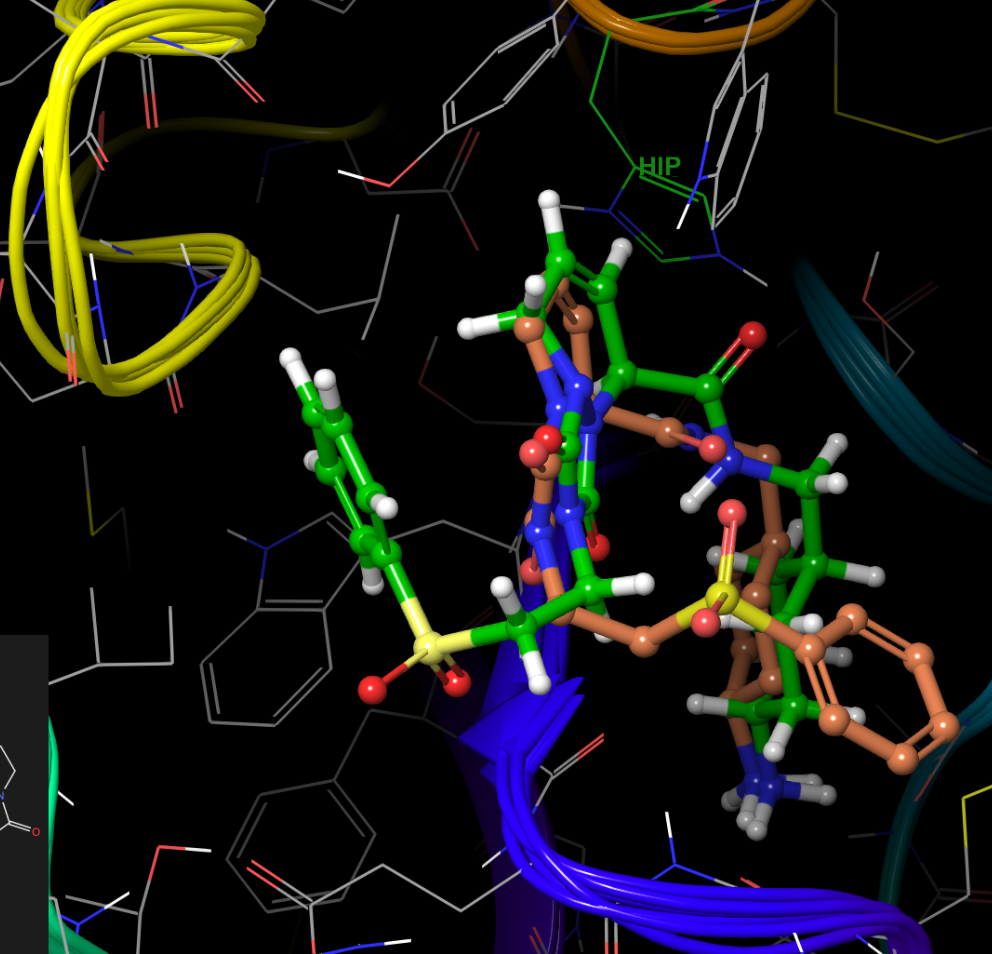
\includegraphics[width=\linewidth]{figures/feature_51_2384.png}
\caption{\footnotesize Pose 2384 (RMSD 5.6Å)}
\end{subfigure}
\hfill
\begin{subfigure}{0.26\linewidth}
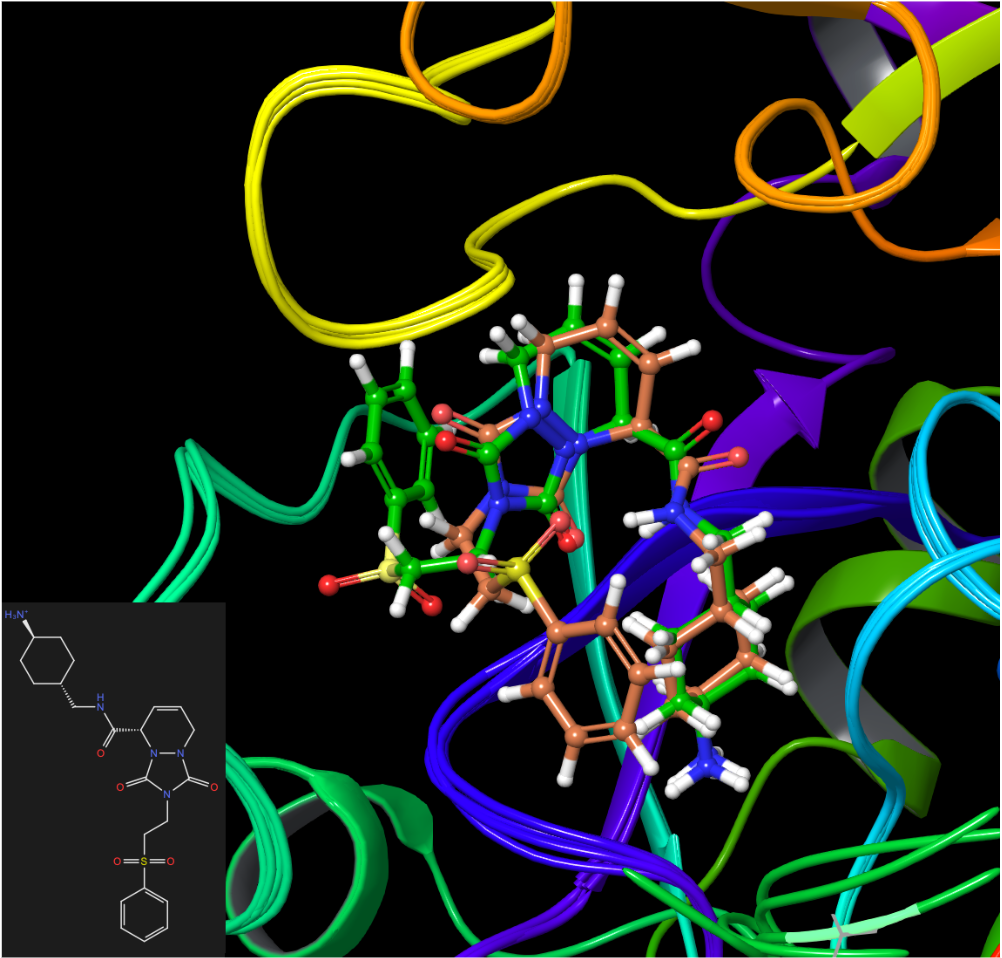
\includegraphics[width=\linewidth]{figures/feature_51_4556.png}
\caption{\footnotesize Pose 4556 (RMSD 7.2Å)}
\end{subfigure}
\hfill
\begin{subfigure}{0.26\linewidth}
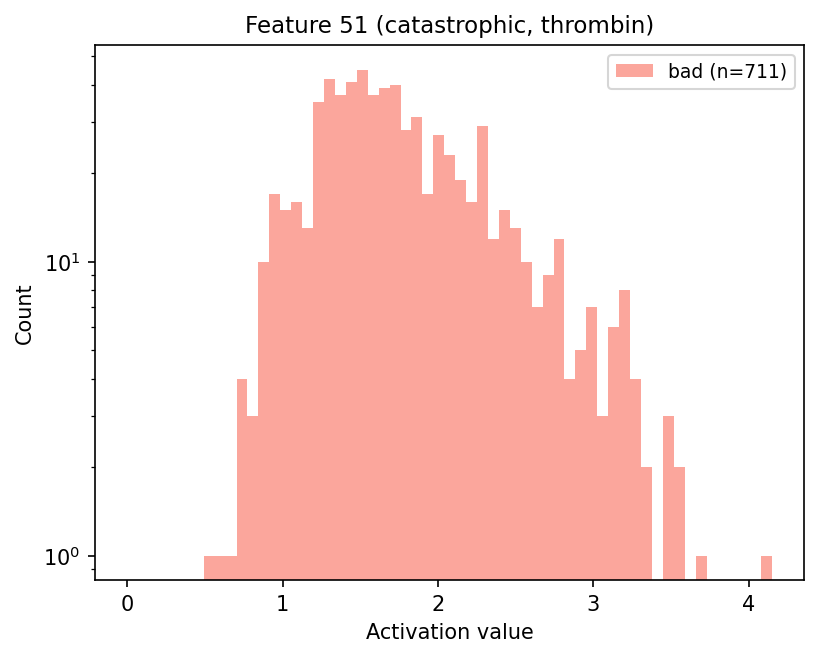
\includegraphics[width=\linewidth]{figures/feature_51_activation_dist.png}
\caption{\footnotesize Activation dist.\ (2Å label)}
\end{subfigure}
\vspace{-6pt}

\begin{subfigure}{0.26\linewidth}
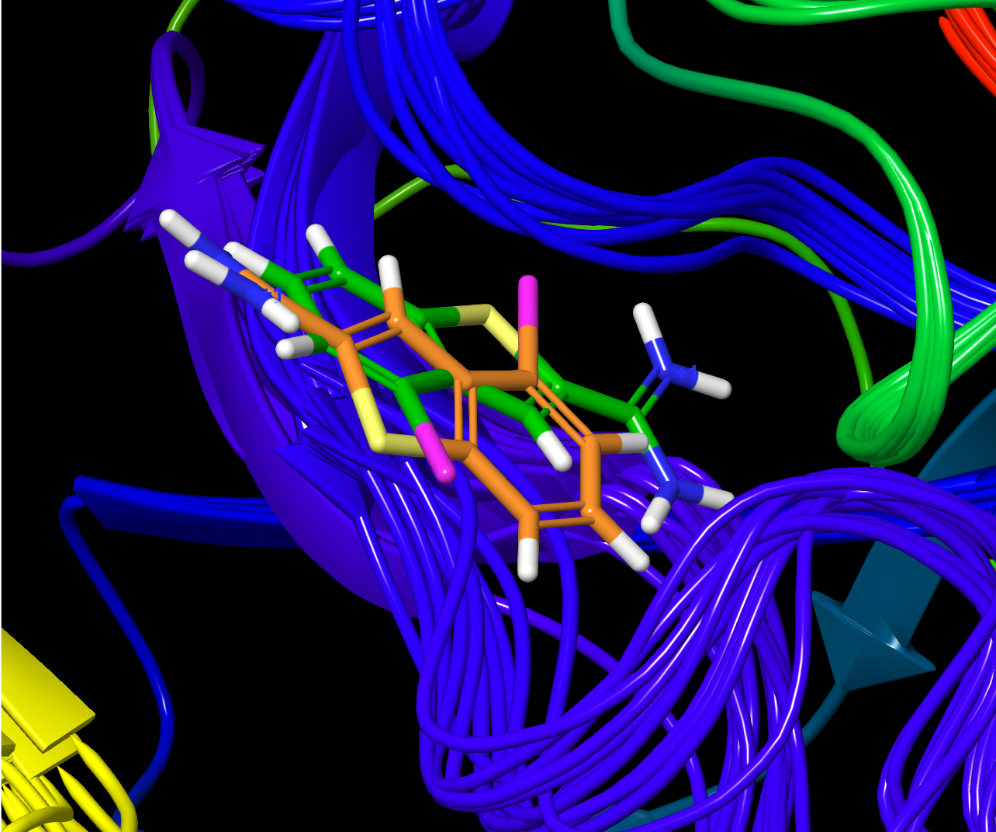
\includegraphics[width=\linewidth]{figures/feature_84_11084.png}
\caption{\footnotesize Pose 11084 (RMSD 5.7Å)}
\end{subfigure}
\hfill
\begin{subfigure}{0.26\linewidth}
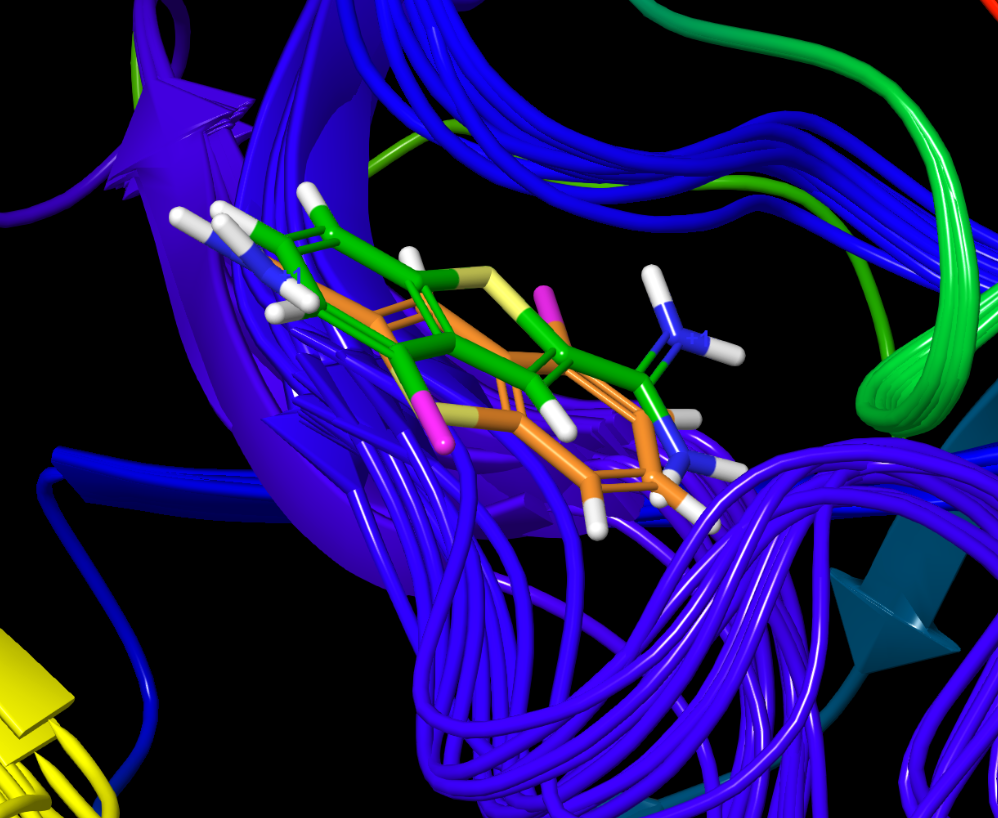
\includegraphics[width=\linewidth]{figures/feature_84_11377.png}
\caption{\footnotesize Pose 11377 (RMSD 5.0Å)}
\end{subfigure}
\hfill
\begin{subfigure}{0.26\linewidth}
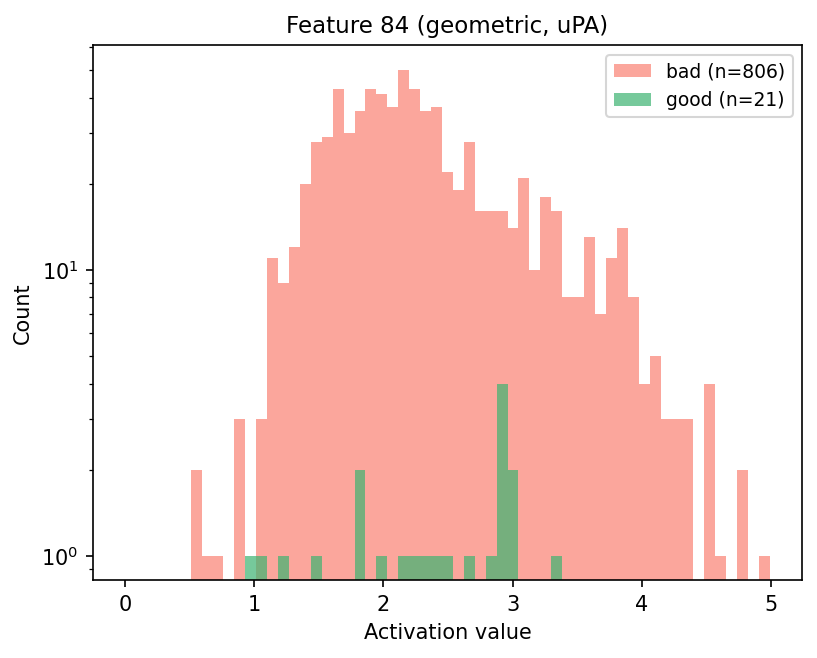
\includegraphics[width=\linewidth]{figures/feature_84_activation_dist.png}
\caption{\footnotesize Activation dist.\ (2Å label)}
\end{subfigure}
\vspace{-2pt}
\caption{\small Feature 51 (top, thrombin) and Feature 84 (bottom, uPA), both members of the deployed $K$=8 4Å combo filter (case details and statistics in text). Left/middle: top-activating test poses, docked pose (orange) vs.\ reference (green); the colored backbone traces in Feature 51's poses reflect the pipeline's induced-fit receptor-loop sampling, present in both good and bad poses for this case (see below). Right: activation distribution (active poses only, log-scale count) split by the 2Å native-pose criterion.}
\label{fig:features}
\end{figure}

Table~\ref{tab:filtering}'s $K$=8 combo filter includes two features with sharply contrasting structural signatures. Feature 51 fires on 711 test poses, 99.3\% of which come from a single thrombin case pair \citep{dicera1995} (PDB 1AE8$\to$1D9I \citep{desimone1997,krishnan2000}, 706/711; a second thrombin pair accounts for the remaining 5), at precision 0.809 with a sentinel rate of 86.4\% against a 38.4\% population baseline. Under the stricter, standard 2Å native-pose criterion, precision is perfect: all 711 flagged poses are non-native (0 false positives). Its highest-activating poses (Figure~\ref{fig:features}) show a consistent rotational failure: the ligand's sterically bulky substituent, which should point toward Leu99, instead points toward Ala190---both residues lining the S1/S2 subsites adjacent to the catalytic triad \citep{bode1989}. This misorientation is severe enough that most flagged poses fall outside any refinable basin, consistent with the elevated sentinel rate.

Feature 84 tells a different story. It fires on 827 poses, 94.3\% concentrated in a single urokinase (uPA) case pair \citep{spraggon1995} (PDB 2VIO$\to$1C5W \citep{frederickson2008,katz2000}, 780/827)---the same catalytic serine-protease fold family as thrombin---at precision 0.911 with a sentinel rate of 28.5\%, \emph{below} the population baseline; at the 2Å native-pose criterion, precision rises to 0.975 (806/827). Its highest-activating poses show the ligand correctly oriented but translationally displaced within the binding pocket; energies converge to real, physically stable values (clustered around $-9{,}300$ to $-9{,}700$ kcal/mol) rather than the sentinel value. On the 20 most confidently native poses for this case (RMSD $<$0.4Å), feature 84's activation is exactly 0.0000---the feature is silent on good poses rather than weakly active everywhere.

Together the two features illustrate a rotational-vs-translational split in the geometric errors the SAE decomposes into distinct, monosemantic features: severe rotational misorientation that falls outside any refinable basin (Feature 51), and milder translational displacement that minimization tolerates (Feature 84)---consistent with the monosemanticity hypothesis that sparse features encode distinct failure phenomena rather than one distributed correlate of pose quality \citep{templeton2024,adams2025,clark2026,bricken2023}.

Two additional checks: a search for the mirror-image case (features preferring native-like poses) found nothing comparably precise or concentrated (best 4Å: 55.3\% precision at 1.6\% recall; best 2Å: 22.2\% at 11.1\% recall), and the induced-fit receptor-loop flexibility visible in Feature 51's poses (Figure~\ref{fig:features}) is not diagnostic---the same spread appears in the case's most confidently native poses.

\section{Conclusion}

We have shown that sparse autoencoders can decompose the latent space of a physics-informed docking pipeline into interpretable, case-specific features---high-precision detectors for distinct failure modes that fire rarely and map to physical phenomena. The deployed combo filters remove a substantial share of poor poses while retaining the large majority of native-like conformations at both thresholds (Section 3.2), beating both a raw-latent-geometry baseline and the pipeline's own energy score, which cannot reach these operating points at all (Section 3.3). SAEs offer a path toward docking pipelines that are not only predictive but mechanistically understood---systems whose failures can be diagnosed, explained, and, eventually, corrected.

That Feature 51 and Feature 84 each concentrate almost entirely in a single case pair suggests the SAE learns protein-specific failure signatures that a global classifier would dilute across cases---SAE-based filters are therefore most valuable when the target protein family is known, complementary to case-agnostic scoring rather than a replacement for it. Recall is modest at both headline operating points, a deliberate precision-first choice rather than a ceiling on detectability. Generalization beyond the 36 systems and two failure modes studied here requires further validation; activation steering, as explored for structure-generation models by FoldSAE \citep{zarzecki2025}, is a natural next step.

\paragraph{Broader Impact}
This work aims to reduce computational cost and improve interpretability in structure-based drug discovery by filtering low-quality docking poses before expensive refinement, and by surfacing which physical failure modes a generative model has and has not learned to represent. Because the method filters and interprets existing poses rather than generating novel molecules, it does not meaningfully lower the barrier to designing novel toxic compounds, the primary dual-use concern in ML-for-drug-discovery work. A more realistic risk is uneven performance: our filters are highly case-specific (Section 3.4), so precision guarantees may not transfer to protein families outside the 36 systems studied here, and over-reliance without periodic validation could disproportionately deprioritize research on rarer disease targets.

\begin{ack}
% TODO: confirm with Friesner Group whether the GPU cluster funding acknowledgment below (Gates Foundation) is accurate before submission.
This work was supported by a Rabi Scholars Program stipend (Columbia University). Computational resources were provided by the Friesner Group's GPU cluster. The docking dataset was generated using Schr\"odinger's IFD-ML pipeline through an academic collaboration with the Friesner Group; the authors declare no financial competing interests.
\end{ack}

\bibliography{references}
\bibliographystyle{plainnat}

\newpage
\input{checklist.tex}

\end{document}
